\begin{center}
\Huge
Den naturlige eksponentialfunktion og logaritme
\end{center}
\stepcounter{section}

\section*{Den naturlige eksponentialfunktion}

Én eksponentialfunktion har så pæne egenskaber, at den fortjener et særligt navn; den naturlige eksponentialfunktion. Vi definerer den her.
\begin{defn}[Den naturlige eksponentialfunktion]
	Den naturlige eksponentialfunktion defineres som funktionen $f$ givet ved
	\begin{align*}
		f(x) = e^x,
	\end{align*}
	hvor $e \approx 2.718281$ kaldes for \textit{Eulers tal.}
\end{defn}
Denne eksponentialfunktion vil vi arbejde med særligt i 2. og 3.g. Den har begyndelsesværdi 1 og opfylder, at hældningen af funktionen alle steder er lig funktionsværdien, hvilket vi dog først vil præcisere næste år. 

Vi kan bruge Eulers tal $e$ til at repræsentere alle eksponentialfunktioner. Vi vil dog først præsentere \textit{den naturlige logaritme}. 

\section*{Den naturlige logaritme}
\stepcounter{section}

På samme måde som vi sidst eksempelvis brugte $\log_2$ i forbindelse med eksponentialfunktionen $2^x$ og $\log_{10}$ i forbindelse med eksponentialfunktionen $10^x$ vil vi her definere den naturlige logaritme, der er den inverse funktion til den naturlige eksponentialfunktion. 
\begin{defn}[Den naturlige logaritme]
	Den naturlige logaritme defineres som logaritmen med grundtal $e$, altså
	\begin{align*}
		\log_e(x).
	\end{align*}
	Denne skrives ofte 
	\begin{align*}
		\ln(x).
	\end{align*}
\end{defn}
Denne opfylder som bekendt, at 
\begin{align*}
	\ln(e^x) = x
\end{align*}
og 
\begin{align*}
	e^{\ln(x)} = x.
\end{align*}
\begin{exa}
	Det gælder eksempelvis, at $\ln(e^{10}) = 10$ og $e^{\ln(4)} = 4$.
\end{exa}

Vi kan bruge den naturlige logaritme og den naturlige eksponentialfunktion til at omskrive alle eksponentialfunktioner.
Har vi en eksponentialfunktion $f$ givet ved
\begin{align*}
	f(x) = b\cdot a^x,
\end{align*}
så kan vi udnytte, at 
\begin{align*}
	a = e^{\ln(a)}
\end{align*}
samt regnereglen 
\begin{align*}
	(a^{y})^x = a^{x\cdot y}.
\end{align*}
Derfor kan vi skrive $a^x$ som
\begin{align*}
	a^x = (e^{\ln(a)})^x = e^{\ln(a)\cdot x}.
\end{align*}
Vi kalder nu $\ln(a) = k$ og indsætter dette i forskriften for $f$. Vi får derfor
\begin{align*}
	f(x) = b\cdot a^x = b\cdot e^{kx}.
\end{align*}
Enhver eksponentialfunktion kan altså omskrives til formen 
\begin{align*}
	f(x) = b\cdot e^{kx},
\end{align*}
hvor $k = \ln(a)$.

\begin{exa}
	Vi ønsker at omskrive eksponentialfunktionen $f$ givet ved
	\begin{align*}
		f(x) = 10\cdot 1.32^x
	\end{align*}
	til formen 
	\begin{align*}
		f(x) = b\cdot e^{kx}.
	\end{align*}
	Vi udnytter, at $k = \ln(a) = \ln(1.32) = 0.278$ og får, at $f$ kan skrives som
	\begin{align*}
		f(x) = 10e^{0.278x}.
	\end{align*}
	Vi kan også være i situationen, hvor vi ønsker at gå den anden vej. Lad os betragte tilfældet, hvor vi har
	fået en eksponentialfunktion $g$ givet ved
	\begin{align*}
		g(x) = 14\cdot e^{-0.11x}.
	\end{align*}		
	Vi kan i denne situation ikke umiddelbart aflæse hverken fremskrivningsfaktor eller vækstrate. For at gøre 
	dette skal vi omskrive $g$ til formen
	\begin{align*}
		g(x) = b\cdot a^x.
	\end{align*}
	Da $k = \ln(a)$, så må det gælde, at $e^k = e^{\ln(a)} = a$, så vi kan altså finde fremskrivningsfaktoren
	$a$ ved at bestemme $a = e^{-0.11} = 0.896$, og $g$ lyder derfor
	\begin{align*}
		g(x) = 14\cdot 0.896^x.
	\end{align*}	
\end{exa} 

\subsection*{Grafer}

Da logaritmer gør det omvendte af eksponentialfunktioner (de er inverse til eksponentialfunktioner), må deres grafer være eksponentialfunktioner spejlet i linjen $y = x$. (Hvis dette ikke er klart, så kommer vi til at vende tilbage til det senere). Grafen for $e^x$ samt $\ln(x)$ kan ses af Figur \ref{fig:ekspln}
\begin{figure}[H]
	\centering
	\begin{tikzpicture}
		\begin{axis}[axis lines = center,		
		xmin = -3, xmax = 5,
		ymin = -3, ymax = 5,
		xlabel = $x$, ylabel = $y$,
		xtick = {1}, ytick = {1}]
			\addplot[color = teal, thick, domain = -4:5, samples = 200] {e^x};
			\addplot[color = olive, thick, domain = 0:5, samples = 200] {ln(x)};		
			\node[color = teal] at (axis cs: 2,4) {$e^x$};
			\node[color = olive] at (axis cs: 4,2) {$\ln(x)$};
		\end{axis}
	\end{tikzpicture}
	\caption{Grafer for funktionerne $e^x$ og $\ln(x)$.}
	\label{fig:ekspln}
\end{figure}




\subsection*{Opgave 1}
En tabel med funktionsværdier for $e^x$ er givet.
\begin{table}[H]
	\centering
	\begin{tabular}{c|c|c|c|c|c|c|c|c|c|c}
		$x$ & -4 & -3 & -2 & -1 & 0 & 1 & 2 & 3 & 4 & 5 \\
		\hline
		$\e^x$ & 0.018 & 0.049 & 0.135& 0.368 & 1 & 2.718 & 7.389 & 20.085 & 54.598 & 148.413
	\end{tabular}
\end{table}
Brug tabellen til at bestemme følgende.
\begin{align*}
	&1) \ \ln(20.085)     &&2) \ \ln(54.598)    \\
	&3) \ \ln(1)     &&4) \  \ln(0.018)		\\
	&5) \ \ln(0.049) &&6) \ \ln(148.413)    
\end{align*}


\subsection*{Opgave 2}
Bestem følgende udtryk 
\begin{align*}
	&1) \ \ln(\e^3)    &&2) \ \ln(\e^{17})   \\  
	&3) \ \ln(\e^{\sqrt{4}})   &&4) \ \ln(\e)     \\  
	&5) \ \ln(1)   &&6) \ \ln(\e^{-0.157})   \\  
\end{align*}

\subsection*{Opgave 3 (Med Maple)}
Omskriv følgende eksponentialfunktioner til formen
\begin{align*}
	f(x) = be^{kx}.
\end{align*}
\begin{align*}
	&1) \ f(x) = 2\cdot 1.2^x   &    &2) \  f(x) = 10\cdot 0.75^x \\
	&3) \ f(x) = 1.93\cdot 2^x   &    &4) \  f(x) = 510 \cdot 1.13^x \\
	&5) \ f(x) = \sqrt{2}\cdot 0.9^x   &    &6) \  f(x) = \cdot (e^{-1.5})^x \\
\end{align*}

\subsection*{Opgave 4}
I Opgave 3 havde $k$ forskellige fortegn. Kan du gennemskue, hvad fortegnet for $k$ betyder for eksponentialfunktionen?

\subsection*{Opgave 5 (Med Maple)}
\begin{enumerate}[label = \roman*)]
	\item En eksponentialfunktion $f$ er givet ved
	\begin{align*}
		f(x) = 5\cdot e^{-0.05x}.
	\end{align*}
	Bestem fremskrivningsfaktoren og vækstraten for $f$. 
	\item En eksponentialfunktion $f$ er givet ved
	\begin{align*}
		f(x) = 17 \cdot e^{0.8x}.
	\end{align*}
	Bestem fremskrivningsfaktoren og vækstraten for $f$. 
	\item En eksponentialfunktion $f$ er givet ved
	\begin{align*}
		f(x) = 9.11\cdot e^{-0.17x}.
	\end{align*}
	Afgør, hvor mange procent $f$ stiger med, hver gang $x$ øges med $1$. 
\end{enumerate}

\subsection*{Opgave 6 (Med Maple)}
I en by er indbyggertallet i år 2000 på $15\TS 621$ personer. I år 2010 er der $20\TS 217$ personer. 
Det antages, at indbyggertilvæksten kan beskrives ved en eksponentiel sammenhæng. 

\begin{enumerate}[label=\roman*)]
	\item Bestem en sammenhæng $f(x) = b \cdot e^{kx}$, der beskriver udviklingen af befolkningen i byen. $x$ 
	skal beskrive år efter år 2000 og $f$ skal beskrive befolkningsantallet i byen. 
\end{enumerate}

\subsection*{Opgave 7}

Følgende er en graf for den naturlige eksponentialfunktion $f(x) = e^x$. 

\begin{figure}[H]
	\centering
	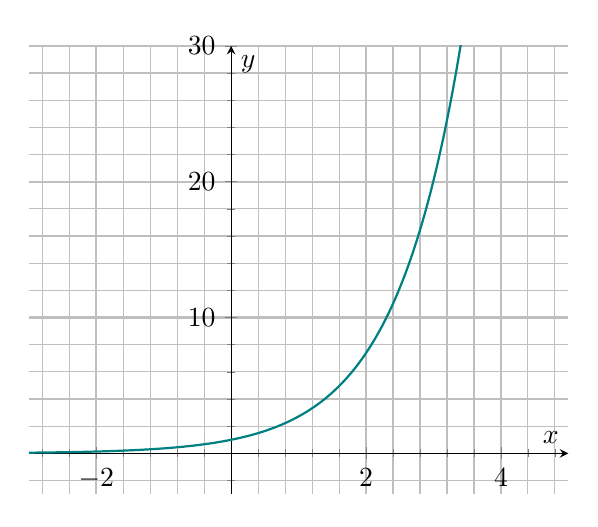
\begin{tikzpicture}
		\begin{axis}[axis lines = center,		
		xmin = -3, xmax = 5,
		ymin = -3, ymax = 30,
		xlabel = $x$, ylabel = $y$,
		grid = both,
		minor tick num = 4,
		major grid style = {thick}
		]
			\addplot[color = teal, thick, domain = -4:5, samples = 200] {e^x};		
		\end{axis}
	\end{tikzpicture}
	\caption{Graf for funktionen $e^x$.}
\end{figure}

Brug grafen for $f(x) = e^x$ til at løse følgende opgaver. Aflæs efter bedste evne. 
\begin{enumerate}[label=\roman*)]
	\item Bestem $e^2$.
	\item Bestem $e^3$.
	\item Bestem $e^{2.6}$.
	\item Bestem $e^0$.
	\item Bestem $\ln(10)$.
	\item Bestem $\ln(20)$.
	\item Bestem $\ln(26)$.
\end{enumerate}


\subsection*{Opgave 8 (Med Maple)}
Løs følgende ligninger både ved brug af $\ln$ og ved brug af solve.

\begin{align*}
	&1)\ e^{x-4} = 403.43 &   &2) \  e^{x/2 - 6} = 54.59\\
	&3)\ \ln(x + 2) = 0.5 &   &4) \ \ln(4x -1) = 3.7  \\
\end{align*}
